\documentclass[11pt]{article}

\usepackage[utf8]{inputenc} % Required for inputting international characters
\usepackage[a4paper]{geometry}
\usepackage[T1]{fontenc} % Output font encoding for international characters
\usepackage[english]{babel}

\usepackage{hyperref}
\usepackage{graphicx}
\usepackage{subcaption}
\usepackage{float}
\usepackage{glossaries}
\usepackage{appendix}
\usepackage{adjustbox}
\usepackage{listings}
\usepackage{xcolor}
\usepackage{fancyhdr}
\usepackage{microtype}
\usepackage{soul} % Underline with wrapped text
\usepackage{multicol}

% Font
\usepackage[proportional,scaled=1.064]{erewhon}
\usepackage[erewhon,vvarbb,bigdelims]{newtxmath}
\renewcommand*\oldstylenums[1]{\textosf{#1}}

\pagestyle{fancy}
\fancyhf{}
\lhead{Functional Programming Project}
\rhead{Sgit}
\lfoot{Thomas Falcone}
\rfoot{\thepage}
\renewcommand{\footrulewidth}{0.4pt}

\definecolor{stringcode}{HTML}{7ec699}
\definecolor{commentcode}{HTML}{999999}
\definecolor{backcolour}{HTML}{002835}

\lstdefinestyle{kuzzleCore}{
    backgroundcolor=\color{backcolour},
    commentstyle=\color{commentcode},
    keywordstyle=\color{magenta},
    numberstyle=\tiny\color{backcolour},
    stringstyle=\color{stringcode},
    basicstyle=\ttfamily\footnotesize\color{white},
    breakatwhitespace=false,
    breaklines=true,
    captionpos=b,
    keepspaces=true,
    numbers=left,
    numbersep=5pt,
    showspaces=false,
    showstringspaces=false,
    showtabs=false,
    tabsize=2
}

\lstset{style=kuzzleCore}

\lstdefinelanguage{Javascript}{
  keywords={break, case, catch, continue, debugger, default, delete, do, else, finally, for, function, if, in, instanceof, new, return, switch, this, throw, try, typeof, var, void, while, with},
  morecomment=[l]{//},
  morecomment=[s]{/*}{*/},
  morestring=[b]',
  morestring=[b]",
  sensitive=true,
  inputencoding=utf8,
  extendedchars=true,
  literate={á}{{\'a}}1 {ã}{{\~a}}1 {é}{{\'e}}1
}

\lstdefinelanguage{Gherkin}{
  keywords={When, Then, Given, And},
  ndkeywords={Feature, Scenario},
  sensitive=false,
  comment=[l]{\#},
  morestring=[b]',
  morestring=[b]"
}
\lstdefinelanguage{scala}{
  morekeywords={%
          abstract,case,catch,class,def,do,else,extends,%
          false,final,finally,for,forSome,if,implicit,import,lazy,%
          match,new,null,object,override,package,private,protected,%
          return,sealed,super,this,throw,trait,true,try,type,%
          val,var,while,with,yield},
  otherkeywords={=>,<-,<\%,<:,>:,\#,@},
  sensitive=true,
  morecomment=[l]{//},
  morecomment=[n]{/*}{*/},
  morestring=[b]",
  morestring=[b]',
  morestring=[b]"""
}[keywords,comments,strings]

\begin{document}

%----------------------------------------------------------------------------------------
%	TITLE PAGE
%----------------------------------------------------------------------------------------

\begin{titlepage} % Suppresses displaying the page number on the title page and the subsequent page counts as page 1
  \newcommand{\HRule}{\rule{\linewidth}{0.5mm}} % Defines a new command for horizontal lines, change thickness here

	\center % Centre everything on the page

	%------------------------------------------------
	%	Headings
	%------------------------------------------------

	\textsc{\LARGE Functionnal Programming project}\\[0.3cm] % Main heading such as the name of your university/college

	\textsc{\Large IT \& Management Department}\\[0.5cm] % Major heading such as course name

	\textsc{\large }\\[0.5cm] % Minor heading such as course title

	%------------------------------------------------
	%	Title
	%------------------------------------------------
	\HRule\\[0.4cm]
	{\huge\bfseries Creation of a Git-like tool in Scala}\\ % Title of your document
	\HRule\\[1.5cm]
	%------------------------------------------------
	%	Author(s)
	%------------------------------------------------

	\begin{minipage}{0.4\textwidth}
		\begin{center}
			\large
			\textit{Author}\\[0.2cm]
			Thomas \textsc{Falcone} % Your name
		\end{center}
	\end{minipage}
	~

	% If you don't want a supervisor, uncomment the two lines below and comment the code above
	%{\large\textit{Author}}\\
	%John \textsc{Smith} % Your name

	%------------------------------------------------
	%	Date
	%------------------------------------------------

	\vfill\vfill\vfill % Position the date 3/4 down the remaining page

	{\large\today} % Date, change the \today to a set date if you want to be precise

	%------------------------------------------------
	%	Logo
	%------------------------------------------------

	\vfill
	$\vcenter{\hbox{
\includegraphics[width=0.35\textwidth]{img/polytech.png}}}$ % Include a department/university logo - this will require the graphicx package
	$\vcenter{\hbox{
\includegraphics[width=0.2\textwidth]{img/ig.png}}}$ % Include a department/university logo - this will require the graphicx package

	%----------------------------------------------------------------------------------------

	\vfill % Push the date up 1/4 of the remaining page

\end{titlepage}

\newpage
\thispagestyle{empty}
\addtocounter{page}{-1}
\tableofcontents
\vfill
\textit{Every link of this document is clickable if you are reading this in a digital format}
\vfill
\clearpage

\section{Instructions}

You can find the source code on Github through the following link : \href{https://github.com/ThomasF34/sgit}{Source code 
\includegraphics[height=\fontcharht\font`\l]{img/github.png}} {\ul{https://github.com/ThomasF34/sgit}}\newline

In order to install \textbf{sgit} you can either use the Github release TODO or build the binary file from the source code. \textit{Be aware that you must have installed sbt before trying to compile the source code. You will find more information about \textit{sbt} on this site \href{https://www.scala-sbt.org/}{https://www.scala-sbt.org/}}\\

To compile from source code use :
\begin{lstlisting}
  sbt assembly
\end{lstlisting}

Then add the file \textit{target/scala-2.13/sgit} to your PATH.\\

To install via the Github release, simply download the binary file and add it to your PATH.\\

\begin{center}
  \textit{You are now able to use sgit. You can find the usage with \textbf{sgit --help}}
\end{center}

\section{Architecture}
\subsection{Presentation}
The architecture of sgit is quite explicit and can be seen as a simple flow.

\begin{figure}[h!]
  \centering
  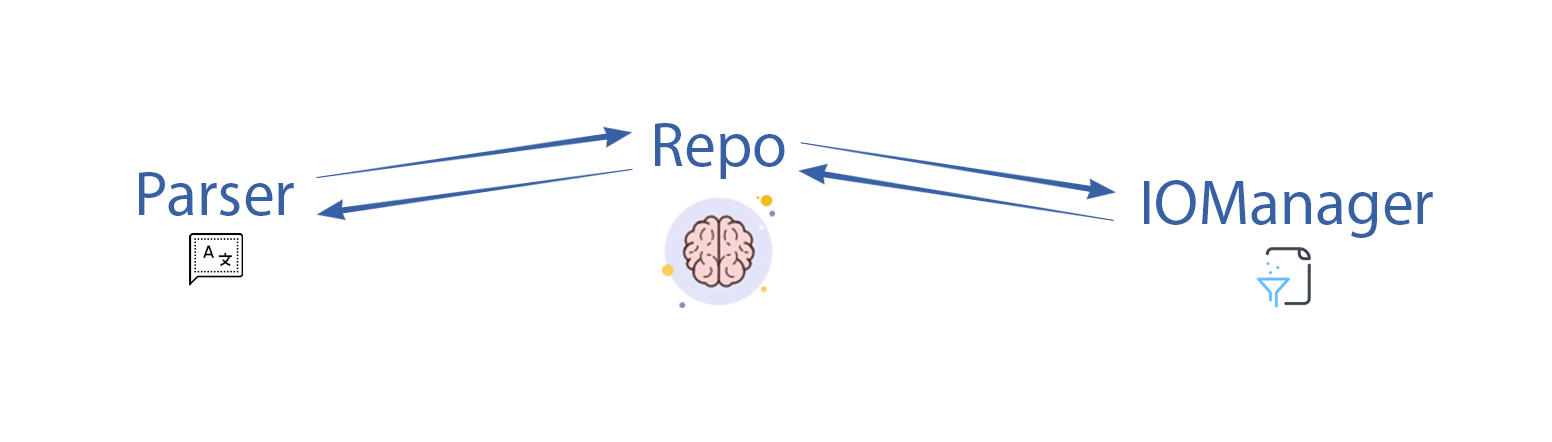
\includegraphics[width=\linewidth]{img/flow.png}
\end{figure}

Everything begins within the \textbf{Parser} that will take the given command, initiate the \textbf{Repo} instance and ask it to execute the wanted action. It will then load all the needed the content from the \textbf{IOManager}, the HQ of File management and compute the result.

In order to achieve this goal, the Repo uses an abstraction of the object it manipulates. Hence, it exists several \textit{case classes} that will help readibility and separate each other's concerns.\\

Here is a list of existing classes :
\begin{multicols}{3}
\begin{itemize}
  \setlength\itemsep{0.1em}
  \item Blob
  \item Tree
  \item Branch
  \item Tag
  \item Commit
  \item Head
  \item Merge
  \item Diff
  \item Change
\end{itemize}
\end{multicols}

Theses objects are using High Order Function in order to gain access to the content they need. For example we give a function called \textit{commitContent} to the Commit object so he can access some commit's information. Hence, every function that need to have a commit information respects Referencial Transparency with this function injection.
The Repo instance is responsible for this function injection. It is using IOManager's function to let other object access file's content, while hiding its origin to the aforementioned object.

\begin{figure}[h!]
  \centering
  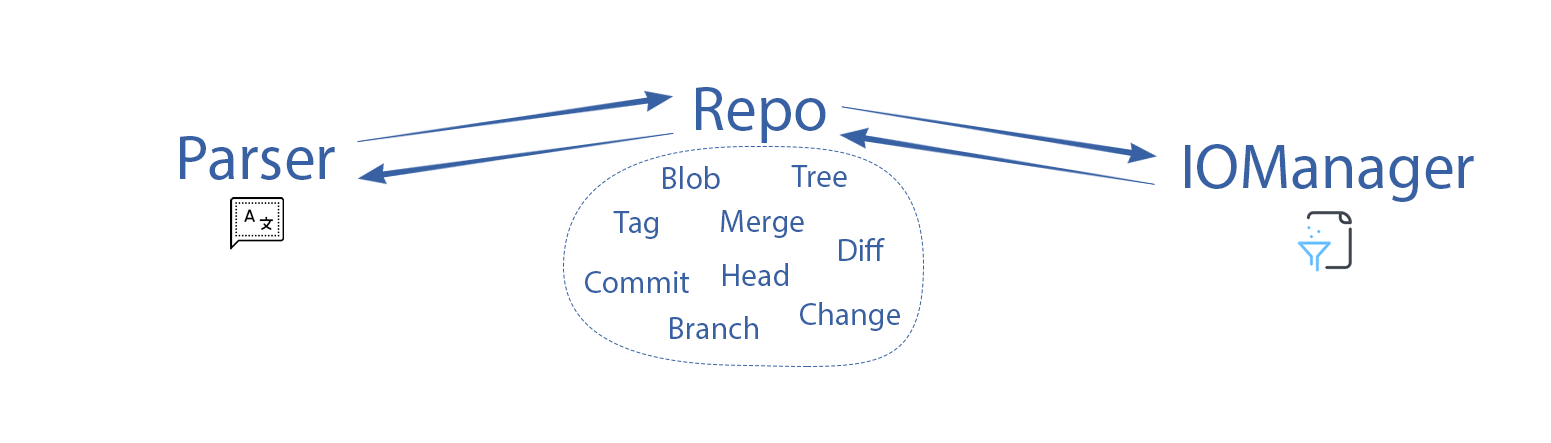
\includegraphics[width=\linewidth]{img/flowDetailled.png}
\end{figure}

Also, I used currying in order to specialize theses functions we are giving to other classes. Let's see how I used currying with an example :

\begin{lstlisting}[language=scala, caption=Function in IOManager]
  def getContent(dir: String)(filename: String): String = {
    val file = new File(s"${dir}$filename")
    if (file.exists() && file.isFile()) {
      Source.fromFile(file).mkString
    } else ""
  }
\end{lstlisting}

\begin{lstlisting}[language=scala, caption=Functions to be injected]
  lazy val blobContent = ioManager.getContent(blobsPath)(_)
  lazy val tagContent = ioManager.getContent(tagsPath)(_)
\end{lstlisting}

With these functions, the Blob instance (to which we are gonna inject \textit{blobContent}) will only be able to access blob content while Tag instance will only be able to access tag content.

\subsection{File organigation}


\subsection{Git copycat}

In order to reproduce most of Git function I had to implement some interesting algorithms.

First for the \textit{diff} functions and then for the \textit{merge} one.

\subsubsection{Diff algorithm}
In order to obtain the diff between two files I implemented an algorithm base on the Longest Common Sequence (LCS) between two collections (here two collection of string where each element represents a line of the compared file)

% TODO %
\subsubsection{Merge algorithm}
To compute the merge algorithm I had to obtain the LCS between three files. The first and the second one are the files on each branch we want to merge and the last one is the file on the common ancestor commit.

I implemented an algorithm to compute the LCS matrix '\textit{in 3D}' and even if it sounds more complex, it is not really the case. In fact, for the merge algorithm we don't need to know if each modified line had been inserted or deleted.

The complex part of this algorithm, though, is \textit{the align} step. I had to align all three file based on their LCS to then compare line by line and apply changes.

Here is an imaged example of what the align step will do. (You can retrieve the algorithm implementation in the \href{https://github.com/ThomasF34/sgit/blob/master/src/main/scala/igpolytech/Merge.scala}{\textit{Merge.scala} file 
\includegraphics[height=\fontcharht\font`\l]{img/github.png}}\footnote{\href{https://github.com/ThomasF34/sgit/blob/master/src/main/scala/igpolytech/Merge.scala}{\ul{https://github.com/ThomasF34/sgit/blob/master/src/main/scala/igpolytech/Merge.scala}}}

\begin{figure}[h!]
  \centering
  \begin{subfigure}[b]{0.4\linewidth}
  \centering
    
\includegraphics[width=0.3\linewidth]{img/tobealigned.png}
    \caption{Before alignment}
  \end{subfigure}
  \begin{subfigure}[b]{0.4\linewidth}
  \centering
    
\includegraphics[width=0.3\linewidth]{img/aligned.png}
    \caption{We can now compare line by line}
  \end{subfigure}
\end{figure}

\subsection{Pros}
% IO is grouped on Repo and IOManager (and Parser for interface displaying)
% Usage of hof to respect RT in all other instanciable object (Commit etc.)
% Usage of currying to limit action of instance
% Usage of lazy val for getters

% Readability with all abstraction
% File readibility in .sgit directory

\subsection{Cons}
% Lot of work with all instanciation
% Repo is a complex object
% Lot of variable to define in Repo to limitate objects actions

\section{Tests}
\subsection{Naïve approach}
% Mainly focused on integration test to see if all use cases were correctly made and all users actions would lead to a successful answer to their needs

% Quickly saw that it was not precise enough to easily catch a problem when it occurs

% After a great refactoring at the end of the project, i changed my point of view on tests and tried more to focus on individuals, unitary tests

\subsection{I-understood-the-mistake approach}
% After spending quite sometime chasing bug, it was obvious to me that unitary tests were much more important than integration one

\section{Post-mortem}
\subsection{Teamwork has a lot of benefits}
\subsection{Testability is important}
\subsection{Dev tools can be a great guiding light}

\end{document}